\documentclass[11pt,a4paper]{jarticle}
\usepackage[dvipdfmx]{graphicx}
\usepackage{url}

\renewcommand{\baselinestretch}{1.05} 
\marginparwidth=0cm
\topmargin=-1cm
\headheight=0.3cm
\headsep=0.7cm
\oddsidemargin=0cm
\evensidemargin=0cm
%\textwidth=43zw
\textwidth=15.92cm
%\textheight=43.3\baselineskip
\baselineskip = 0.5744cm
\textheight=43\baselineskip

\itemsep=0.05\baselineskip
\parsep=0pt
\topsep=0.01\baselineskip
\partopsep=0pt
\listparindent=0zw

%% header and footer
\usepackage{fancyhdr}
\pagestyle{fancy}
\lhead{2014年度 春学期授業}
\chead{インタラクティブ・アート実習}
\rhead{担当教員: 松下 光範}
\cfoot{\thepage}
\renewcommand{\headrulewidth}{0pt}
\renewcommand{\footrulewidth}{0pt}

\usepackage{ascmac}
\usepackage{listings,jlisting}
\usepackage{color}
\definecolor{OliveGreen}{cmyk}{0.64,0,0.95,0.40}
\definecolor{colFunc}{rgb}{1,0.07,0.54}
\definecolor{CadetBlue}{cmyk}{0.62,0.57,0.23,0}
\definecolor{Brown}{cmyk}{0,0.81,1,0.60}
\definecolor{colID}{rgb}{0.63,0.44,0}
\definecolor{rulesepcolor}{gray}{0.666}
\lstset{
  language=Java,%プログラミング言語によって変える。
  basicstyle={\ttfamily\small},
  keywordstyle={\color{OliveGreen}},
  %[2][3]はプログラミング言語によってあったり、なかったり
  keywordstyle={[2]\color{colFunc}},
  keywordstyle={[3]\color{CadetBlue}},%
  commentstyle={\color{Brown}},
  %identifierstyle={\color{colID}},
  stringstyle=\color{blue},
  tabsize=2,
  %frame=trBL,
  %numbers=left,
  numberstyle={\ttfamily\small},
  breaklines=true,%折り返し
  %backgroundcolor={\color[gray]{.95}},
  framexleftmargin=0mm,
  frame=single,
  rulesepcolor=\color{rulesepcolor},
  captionpos=b
}


%%%%%%%%%%%%%%%%%%%%%%%%%%%%%%%%%%%%%%%%%%%%%%%%%%%%%%%%%%%%%%%%
\begin{document}

% title
% \section*{\LARGE{第2講 プログラムと I/O モジュールを組み合わせる}}
\section*{\LARGE{第2講 プログラムからLEDを制御する}}
Processing を使って簡単な絵を書く。
 Arduino を組み合わせる。

%%%%%%%%%%%%%%%%%%%%%%%%%%%%%%%%%%%%%%%%%%%%%%%%%%%%%%%%%%%%%%%%


\section{Processing とは}
Processing\footnote{\url{http://processing.org/}} は、Casey Reas と Benjamin Fry によるオープンソースプロジェクトであり、かつてはMITメディアラボで開発されていた。
電子アートとビジュアルデザインのためのプログラミング言語であり、統合開発環境 (IDE) である。 視覚的なフィードバックが即座に得られるため、初心者がプログラミングを学習するのに適しており、電子スケッチブックの
基盤としても利用できる。
Javaを単純化し、グラフィック機能に特化した言語といえる。

\begin{flushright}
 -wikipedia-
\end{flushright}

% \subsection*{Processing の開発環境}
% Processing のアイコンをダブルクリックすると、統合開発環境 (IDE) が立ち上がる。

\begin{figure}[h]
 \centering
 \includegraphics[width=0.5\columnwidth]{img/processing_ide.eps}
 \caption{Processing の IDE (統合開発環境)}
\end{figure}


\section{Processing の基礎}
以下で、Processing による基本的なプログラミングの説明を行います。
なお、メニューバーの「Help → Reference」でインターネットブラウザが起動し、より詳しい説明が確認できますので、そちらも参考にしてください。
ただし、英語表記です。
Processing にはあらかじめサンプルコード (お手本になるプログラム) が、たくさん用意されているので、それを動かしてみてどんなことができるかを見ておくのも良いかもしれません。
サンプルコードは、メニューバーの「File → Example」から見ることができます。

% \subsection*{Processing の基礎}
% \begin{lstlisting}
%  void setup() {
%    // プログラム開始時に一度だけ実行
%  }

%  void draw() {
%    // setup() の後、プログラムが終わるまで繰り返される
%  }
% \end{lstlisting}

\subsubsection*{初期化とループ処理}
プログラムの一番最初に行われる処理のことを「初期化」という。Processingでは setup という関数で初期化が行われる。

Processing のプログラムで、メインの処理を行う。自分で終わることを宣言する、stopボタン
を押して中断する、エラーになるかしない限り、プログラムの実行は終わらずに、Processingは
draw関数を実行し続ける。

\begin{lstlisting}
 void setup(){
   // 初期化の処理をここに書く
   // プログラム開始時に1度だけ実行される
 }

 void draw(){
   // 繰り返したい処理をここに書く
   // setup()が実行された後にプログラムが終了するまで繰り返される
 }
\end{lstlisting}


\begin{itemize}
 \item \textbf{ウインドウサイズの指定}

       size(w, h);
       w = ウィンドウの幅(px)
       h = ウィンドウの高さ(px)

       setup() の中でしか使ってはいけません。
       
 \item \textbf{カラーモードの設定}

       colorMode(RGB, 256);
       RGB = 赤・緑・青の組み合わせ (Red, Green, Blue)
       256 = 色の範囲を256階調(段階)で指定

 \item \textbf{図形の原点指定}

       rectMode(CORNER);
       CORNER = 四角形の左上が原点 (デフォルト)
       CENTER = 四角形の中心が原点
       ※似たような設定に
       ellipseMode(円の原点指定), imageMode(画像の原点指定)の設定がある。
\end{itemize}



\begin{itemize}
 \item \textbf{線を書く}

       line(x1, y1, x2, y2);
       x1 = 始点のx座標 y1 = 始点のy座標
       x2 = 終点のx座標 y2 = 終点のy座標

 \item \textbf{三角形を書く}

       triangle(x1, y1, x2, y2, x3, y3);
       x1 = 角1のx座標 y1 = 角1のy座標
       x2 = 角2のx座標 y2 = 角2のy座標
       x3 = 角3のx座標 y3 = 角3のy座標

 \item \textbf{四角形を書く}

       rect(x, y, sx, sy);
       x = 原点のx座標 y = 原点のy座標
       sx = 四角形の幅 sy = 四角形の高さ

 \item \textbf{円を書く}

       ellipse(x, y, sx, sy);
       x = 原点のx座標 y = 原点のy座標
       sx = 円の幅 sy = 円の高さ

 \item \textbf{図形に色をつける}

       fill(r, g, b);
       r = Red の値  g = Green の値  b = Blue の値
       fill(value);
       value = r, g, b に同じ値を代入する

 \item \textbf{色を消す}

       noFill();
       
 \item \textbf{縁取り線に色をつける}

       stroke(r, g, b);
       stroke(value);
       色の指定方法は fill と同じ

 \item \textbf{縁取り線の幅を調節する}
       
       strokeWeight(value);
       value = 線の太さ(px)の指定

 \item \textbf{縁取り線を消す}

       noStroke();

 \item \textbf{図形の縁をなめらかにする}

       smooth();

 \item \textbf{ウィンドウの背景色を指定する}

       background(r, g, b);
       background(value);
       色の指定方法は fill と同じ
\end{itemize}



\subsection*{TRY1}
Processing で 本日行う実習のベースとなるプログラムを作成する。
\begin{enumerate}
 \item ウィンドウサイズが 幅が 300ピクセル、高さが 300ピクセル
 \item カラーモードは RGB の 256 階調
 \item ウィンドウの背景色は黒
 \item タテが 200 ピクセル、ヨコが 200 ピクセル の 白い円が、ウインドウの中心に表示される
\end{enumerate}
\begin{flushright}
 (時間のある人は、色々と改造してみましょう。) 
\end{flushright}

\begin{lstlisting}
 void setup(){
   size(??? , ???);
   colorMode(RGB, ???);
   ellipseMode(CENTER);
   background(???);
 }
 
 void draw(){
   background(???, ???, ???, ???);
 }
\end{lstlisting}

\begin{flushright}
 ヒント: ??? には数字が入ります
\end{flushright}


\subsection*{Processing で マウスのクリックを検出する}
Processing では、「mousePressed」という命令文を用いることで、マウスのクリック動作
を簡単に検出することができる。
\begin{lstlisting}
 if (mousePressed == true){
   // マウスボタンを押した時の処理
 } else {
   // マウスボタンを離した時の処理
 }
\end{lstlisting}

\subsection*{TRY2}
 TRY1で作ったプログラムを改造し、マウスが押されたときにPCに図形が表示されるようにする。
Gainer mini を Processing で 使えるようにするライブラリのインポート
 Processing で Gainer mini を利用するには、ライブラリと呼ばれるプログラムのパーツを用
いて Processing の機能を拡張する必要がある。Processing のメニューバーの中の Sketch →
Import Library → gainer を選択すると、今書いているプログラムの一番初めに、ライブラリ
を読み込むための命令文 import processing.gainer.* が書き込まれる。
Gainerオブジェクトの作成
上で挿入されたインポート文のすぐ下に
Gainer gainer;
void setup() 内に、
gainer = new Gainer(this);
Gainer mini の ボタンを利用する
if (gainer.buttonPressed){
<< Gainer mini のボタンが押された時の処理 >>
}


\subsection*{TRY3}
 TRY2で作ったプログラムを改造し、Gainer mini のボタンが押された時に、PCに図形が表示
されるようにする。

Gainer mini のdigital output を利用する
digital output (ON, OFF の切り替え)
 digital output を利用することで、Processing 上から、Gainer mini に流れる電流の ON 、
OFF を制御することができる。
ONにしたい場合
gainer.setHigh(0);
(※数字部分は dout のピン番号)
OFFにしたい場合
gainer.setLow(0);
(※数字部分は dout のピン番号)

\subsection*{TRY4}
 TRY3で作ったプログラムに命令文を追加して、Gainer mini のボタンが押された時に、dout 0
に接続したLEDが光るようにする。


\begin{figure}[h]
 \centering
 \includegraphics[width=0.5\columnwidth]{img/circuit.eps}
\end{figure}






\end{document}